\documentclass{standalone}
\usepackage{tikz}
\usepackage{pgfplots}
\pgfplotsset{compat=1.18}
\begin{document}

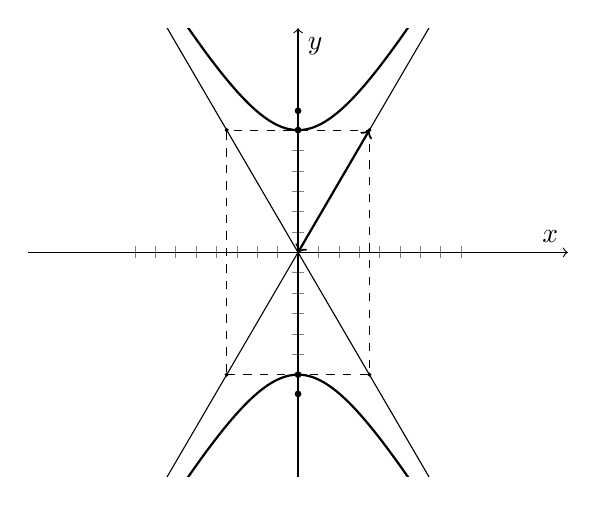
\begin{tikzpicture}[scale=1]
\begin{axis}[
    xmin=-7.5, xmax=7.5,
    ymin=-11, ymax=11,
    axis lines=middle,
    axis line style={->},
    ticklabel style={font=\tiny},
    axis equal,
    xtick={-8,-7,-6,-5,-4,-3,-2,-1,0,1,2,3,4,5,6,7,8},
    ytick={-5,-4,-3,-2,-1,0,1,2,3,4,5},
    xticklabels=\empty,
    yticklabels=\empty,
    xlabel={$x$},
    ylabel={$y$}
]

% Parameters
\def\a{3.5}
\def\b{6}
\pgfmathsetmacro{\c}{sqrt(\a*\a + \b*\b)} % c = 5

% Hyperbola
\addplot [domain=-1.5:1.5, samples=200, thick] 
    ({\a*sinh(x)}, {\b*cosh(x)});
\addplot [domain=-1.5:1.5, samples=200, thick] 
    ({\a*sinh(x)}, {-\b*cosh(x)});

% Asymptotes (solid lines)
\addplot [domain=-8:8] {(\b/\a)*x};
\addplot [domain=-8:8] {-(\b/\a)*x};

% Conjugate rectangle (dashed)
\addplot [dashed] coordinates {
    (-\a,-\b)
    (\a,-\b)
    (\a,\b)
    (-\a,\b)
    (-\a,-\b)
};

% Foci
\filldraw (axis cs:0,\c) circle (1pt);
%\node[above] at (axis cs:0,\c) {$c$};
\filldraw (axis cs:0,-\c) circle (1pt);
%\node[above] at (axis cs:0,-\c) {$-c$};

% Vertices
\filldraw (axis cs:0,\b) circle (1pt);
%\node[above ] at (axis cs:\a,0) {$b$};
\filldraw (axis cs:0,-\b) circle (1pt);
%\node[above ] at (axis cs:-\a,0) {$-b$};

\filldraw (axis cs:-\a,-\b) circle (0.5pt);
\filldraw (axis cs:\a,\b) circle (0.5pt);
\filldraw (axis cs:-\a,\b) circle (0.5pt);
\filldraw (axis cs:\a,-\b) circle (0.5pt);

%\node[ left] at (axis cs:0,\b) {$a$};
%\node[ left] at (axis cs:0,-\b) {$-a$};
\draw[<->, thick] (axis cs:0,0) -- (axis cs:\a,\b);% node[midway, above] {$c$};
\end{axis}
\end{tikzpicture}

\end{document}